\documentclass{article}
\usepackage{graphicx}
\usepackage{polski}
\usepackage[utf8]{inputenc}
\usepackage{graphicx}

\usepackage{subcaption}
\usepackage{algpseudocode}
\usepackage{amssymb}
\usepackage{listings}

\usepackage[a5paper]{geometry}
\graphicspath{ {./wykresy/} }
\begin{document}
\title{Model Chandrasekhara / Smoluchowskiego  - 2 pudła}
\author{Piotr Piękos}

\maketitle

W tym przypadku rozpatrujemy przypadek z dwoma pudełkami. 

Osoba "rodzi się" na podstawie procesu Poissona z częstotliwością $a_N$ trafiając do pudełka 1, spędza tam czas będący zmienną losową o rozkładzie wykładniczym z parametrem $a_{S_1}$. Następnie przechodzi do drugiego pudełka w którym spędza czas będący zmienną losową o rozkładzie wykładniczym z parametrem $a_{S_2}$
\section{Prawa Ewolucji}

Prawa ewolucji są naturalnym rozszerzem praw ewolucji z procesu dla jednego pudełka. W szczególności pierwsze pudełko musi operować na dokładnie tych samych zasadach co poprzednio.

\[P(X_1(t+h) = x_1 + 1, X_2(t+h)=x_2 | X_1(t) = x_1, X_2(t) = x_2) = a_N h + o(h)\]
\[P(X_1(t+h) = x_1 - 1, X_2(t+h)=x_2 + 1| X_1(t) = x_1, X_2(t) = x_2) = a_{S_1} xh + o(h)\]
\[P(X_1(t+h) = x_1, X_2(t+h)=x_2 - 1| X_1(t) = x_1, X_2(t) = x_2) = a_{S_2} xh + o(h)\]
\[P(X_1(t+h) = x_1, X_2(t+h)=x_2| X_1(t) = x_1, X_2(t) = x_2) = 1 - (a_{S_1}  + a_{S_2})xh + o(h)\]
dla każdego innego przejścia prawdopodobieństwo to $o(h)$

Przy naturalnych założeniach $x_1 > 0$ lub $x_2 > 0$ kiedy się zmniejsza.

\section{Algorytm}

Algorytm jest naturalnym rozszerzeniem algorytmu symulacji jednego pudełka



\begin{algorithmic}
\State Gen $N \sim \textit{Poiss}(a_Nt)$
\State for $i = 1$ to N do Gen $U_i \sim U(0, t)$, Gen $L1_i \sim \textit{Exp}(1/a_{S_1})$, Gen $L2_i \sim \textit{Exp}(1/a_{S_2})$
\State $(T_1, ..., T_n) =$ Sort$(U_1, ..., U_n)$ otrzymujemy proces Poissona, czasy narodzin
\State $(D1_1, ..., D1_n) = (T_1 + L1_1, ..., T_n + L1_n)$ - dodajemy niezalezne czasy zycia do czasow narodzin i mamy czasy przejscia do drugiego pudelka.
\State $(D2_1, ..., D2_n) = (D1_1 + L2_1, ..., D1_n + L2_n)$ - dodajemy niezalezne czasy zycia do czasow narodzin i mamy czasy smierci.
\end{algorithmic}  

Czyli od poprzedniego algorytmu różni się jedynie tym że losujemy dodatkowo czasy przebywania w drugim pudełku.

\section{Przykładowe trajektorie}

\begin{figure}[!htb]
\centering
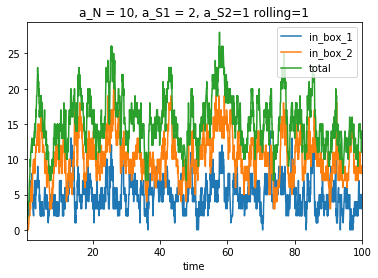
\includegraphics[width=0.4\linewidth]{10,1,2}
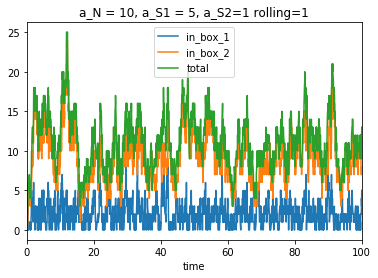
\includegraphics[width=0.4\linewidth]{10,5,1}
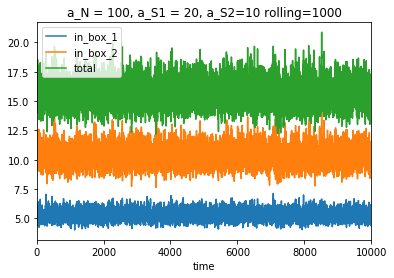
\includegraphics[width=0.4\linewidth]{10,20,10,1000}
\caption{Przykładowe trajektorie symulacji. Dwie górne to niewygładzone trajektorie dla $t=100$. Na niewygładzonych trajektoriach o wiele lepiej widać relację między ilością elementów w jednym i drugim pudełku. Na rysunkach widać ilość elementów w pierwszych pudełku (niebieska linia), ilość elementów w drugim pudełku (pomarańczowa linia) i łączna ilość (suma) elementów (zielona linia). Na dolnym wykresie przedstawiona jest trajektoria symulacji o $t=10000$ z wygładzeniem 1000 (przedstawiona średnia krocząca = 1000) ma ona bardzo podobny kształt do trajektorii z jednym pudełkiem z odpowiadającymi intensywnościami.}
\end{figure}
Wygenerowane wykresy są sparametryzowane 4 parametrami: \begin{itemize}
\item $t$ - długość symulacji
\item $a\_N - a_N$
\item $a\_S - a_S$
\item rolling - długość horyzontu średniej kroczącej, średnia krocząca jest konieczna dla wielu wykresów ze względu na ogromną ilośc punktów na wykresie. Pokazuje jednak ona "gęstość" punktów.
\end{itemize}
\newpage
\section{Rozkład}

Zacznijmy od wartości oczekiwanych. Licząc podobnie jak dla pojedynczego pudełka mozna zauważyć, że 

\[\lim_{t\rightarrow \infty}\mathbb{E}X_1 = \frac{a_N}{a_{S1}} \]
\[\lim_{t\rightarrow \infty}\mathbb{E}X_2 = \frac{a_N}{a_{S2}} \]

Zgadza sie to z oczekiwaniami:
$X_1$ zachowuje się dokładnie tak samo jak w przypadku jednego pudła, więc wynik jest ten sam. $\mathbb{E}X_2$ bierze się stąd, że pierwsze pudło jedynie opóźnia trafienie cząstek do pudełka 2. Czyli można na to patrzeć również jak na model z jednym pudłem tylko teraz cząstka rodzi się z intensywnością $a_N$. Nastepnie czeka jakiś czas (czekanie spowodowane pierwszym pudełkiem) i trafia do pudełka numer 2. Czekanie nie wpływa jednak na średnią ilość cząstek będących w pudełku numer 2.

\subsection{Estymacja kowariancji}

Kowariancję estymujemy ze wzoru \[COV(X,Y) = \mathbb{E}XY - \mathbb{E}X \mathbb{E}Y \] Umiemy policzyć $\mathbb{E}Y i \mathbb{E}X$. Potrzebujemy jedynie $\mathbb{E}XY$ które liczymy w ten sam sposób - ważąc długością występowania danej wartości. Czyli \[\hat{COV(X,Y)} = \hat{\mathbb{E}XY} - \hat{\mathbb{E}X} \hat{\mathbb{E}Y}\]

Generuje to problemy z obciążeniem, (stopnie swobody estymatora wariancji). Jednak skorzystamy tutaj zgodności i oszacujemy to za pomocą dostatecznie dużej próbki, żeby obciążenie było zaniedbywalne

Po symulacjach z różnymi parametrami doszedłem do wniosku, że zawartości pudełek są nieskorelowane, tzn \[COV(X,Y) = 0\]


\section{Uruchamianie symulacji}
\noindent kod do uruchamiania symulacji - w folderze dwa\_pudla:
\begin{lstlisting}[language=bash]
  $ python3 sym.py t a_N a_S1 a_S2 output_file 
\end{lstlisting}
gdzie: \begin{itemize}
\item t - czas trwania symulacji
\item a\_N - intensywność procesu narodzin
\item a\_S1 - Parametr rozkładu czasu przebywania w pierwszym pudle
\item a\_S2 - Parametr rozkładu czasu przebywania w drugim pudle
\item output\_file - nazwa pliku do którego ma się zapisać symulacja (csv)
\end{itemize}

wykresy zostały stworzone w notebooku (dwa\_pudla/)simulate.ipynb
\end{document}